\documentclass{article}
\usepackage{graphicx, amsmath}
\graphicspath{ {./images/} }


\title{Supply \& Demand Together Problem Set Solutions}
\author{Principles of Microeconomics}
\date{\today}

\begin{document}

\maketitle

\begin{enumerate}

\item (b)
	\begin{figure}[h]
	\centering
	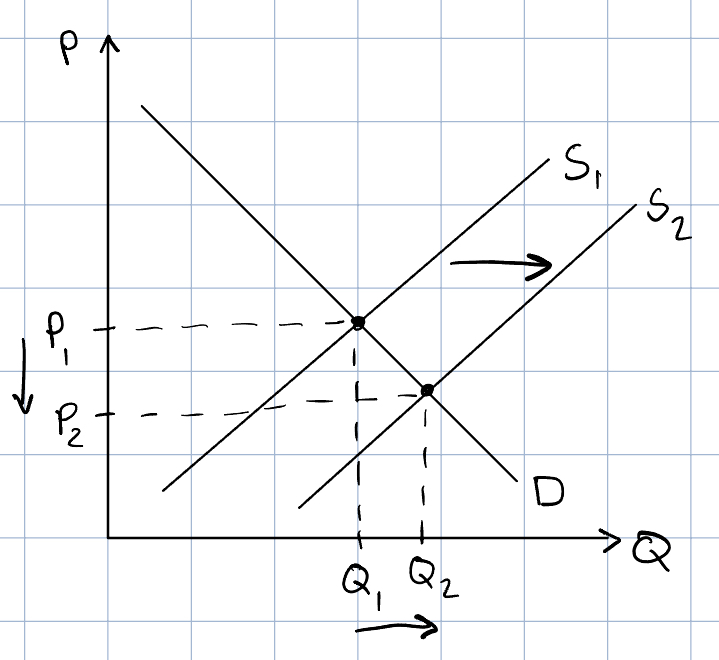
\includegraphics[width = 0.5\textwidth]{problem1}
	\end{figure}

\item (a)
	\begin{figure}[h]
	\centering
	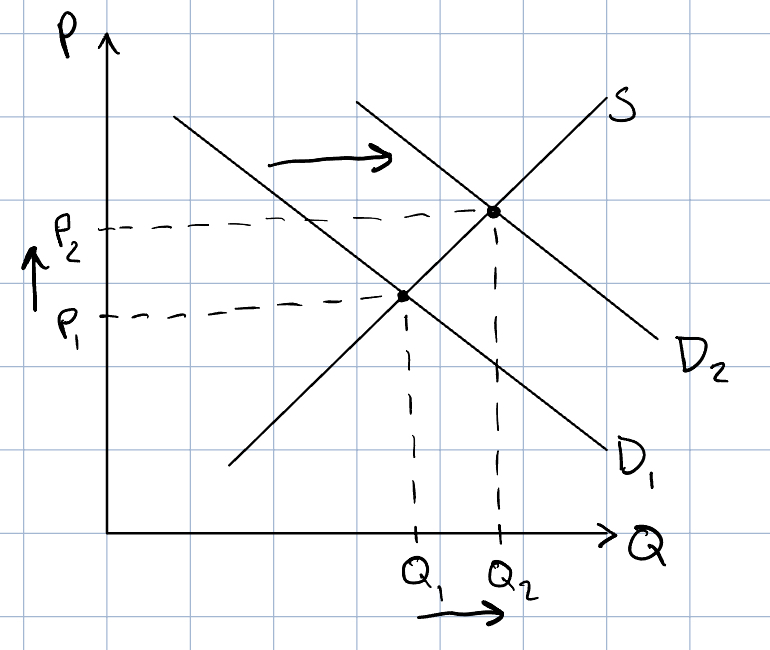
\includegraphics[width = 0.5\textwidth]{problem2}
	\end{figure}

\item (c) -- For equilibrium price to increase and quantity to decrease, we need supply to shift left. That happens when input prices increase.
	\begin{figure}[h]
	\centering
	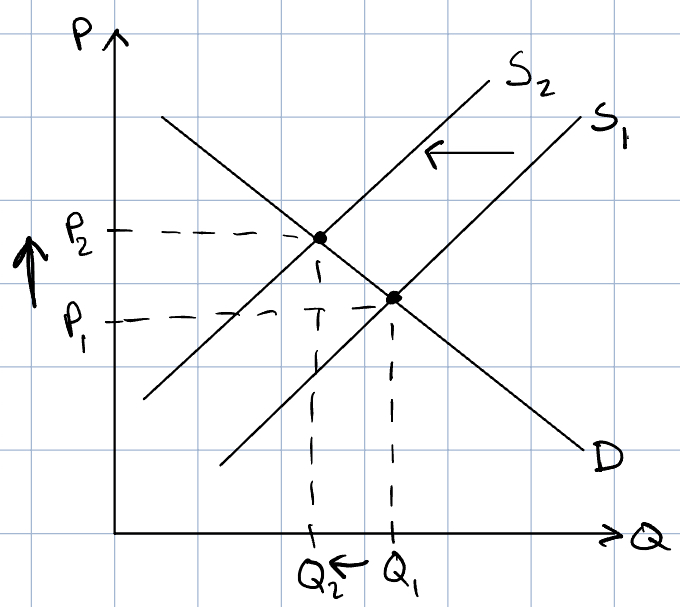
\includegraphics[width = 0.5\textwidth]{problem3}
	\end{figure}

\item Supply remains the same while demand shifts left which causes quantity supplied, quantity demanded, and price to all decrease. Recall that quantity supplied and quantity demanded are both equal to the equilibrium quantity. 
	\begin{figure}[h]
	\centering
	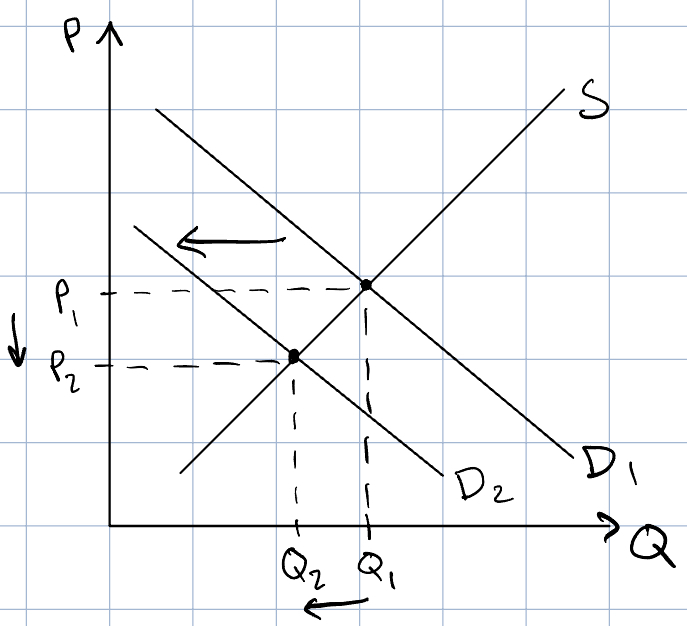
\includegraphics[width = 0.5\textwidth]{problem4}
	\end{figure}
	
\newpage

\item
	\begin{enumerate}
	
	\item The cold snap will increase the cost of oranges, an input to OJ, which shifts the supply curve left and increases the equilibrium price. 
	\begin{figure}[h]
	\centering
	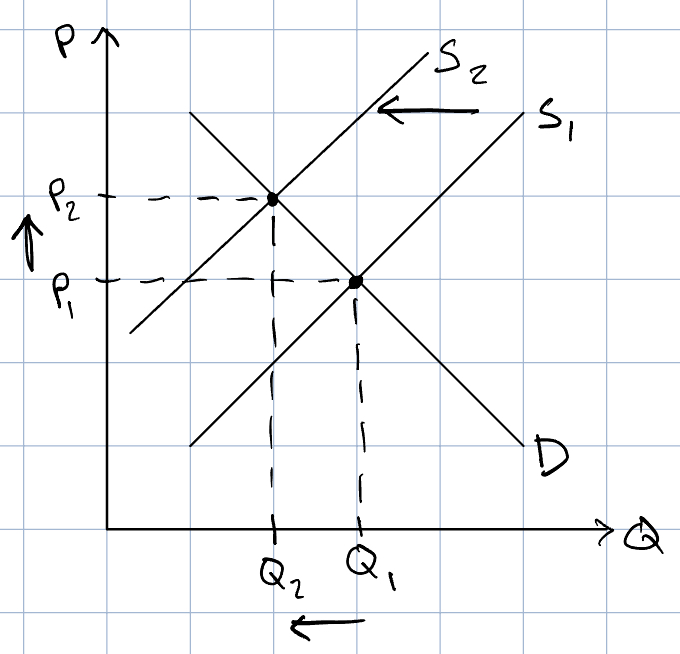
\includegraphics[width = 0.5\textwidth]{problem5a}
	\end{figure}

	
	\item People's preferences for hotel rooms move away from the Caribbean which decreases demand and drives down the equilibrium price.
	\begin{figure}[h]
	\centering
	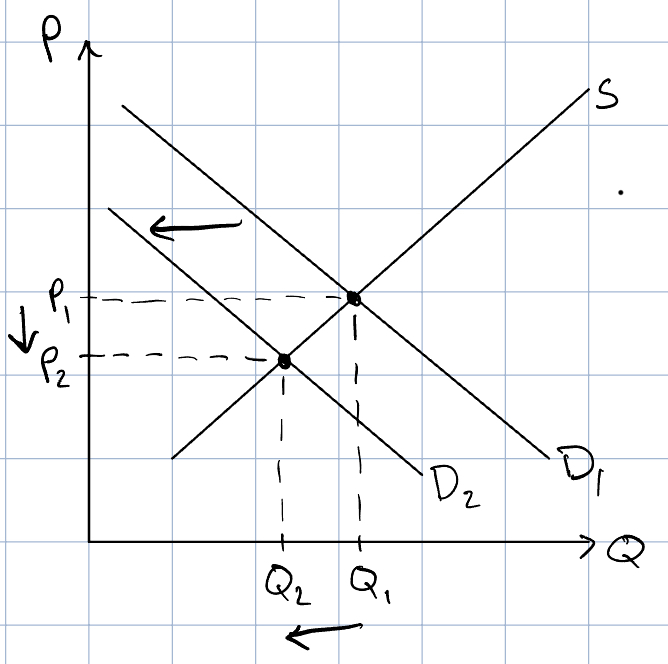
\includegraphics[width = 0.5\textwidth]{problem5b}
	\end{figure}
	
	\newpage
	
	\item When war breaks out in the middle east, the cost of oil increases which increases the price of gasoline. Gasoline and cars are complements, so when the price of gasoline goes up, demand for cars shifts left and the price of cars drops.
	\begin{figure}[h]
	\centering
	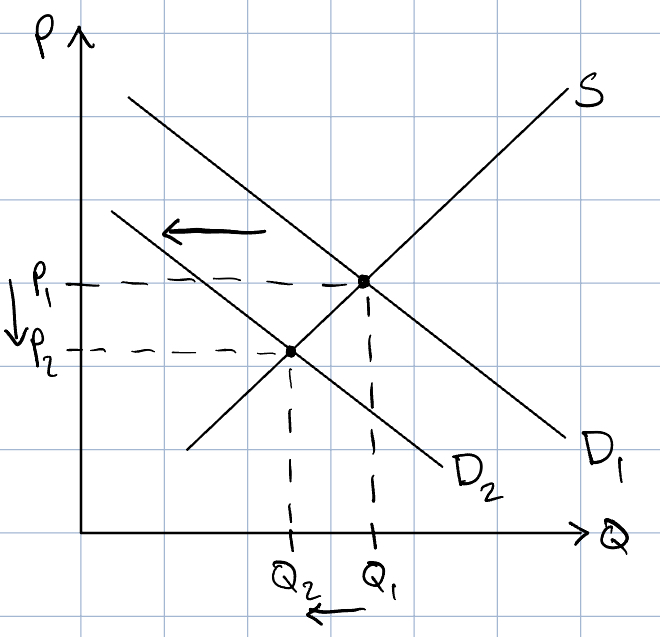
\includegraphics[width = 0.5\textwidth]{problem5c}
	\end{figure}
	
	\end{enumerate}
	
\item

	\begin{enumerate}
	
	\item Having more children will increase people's preferences for minivans and shift demand to the right. That increases the equilibrium price and quantity of minivans.
	\begin{figure}[h]
	\centering
	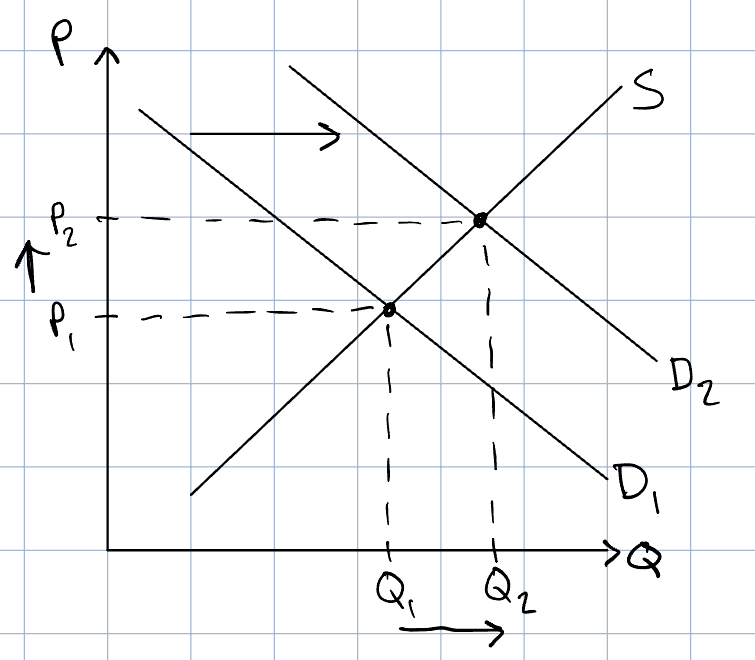
\includegraphics[width = 0.5\textwidth]{problem6a}
	\end{figure}	
	
	\newpage
	
	\item An input price has increased, so the supply of minivans will shift to the left. That increases equilibrium price and decreases equilibrium quantity.
	\begin{figure}[h]
	\centering
	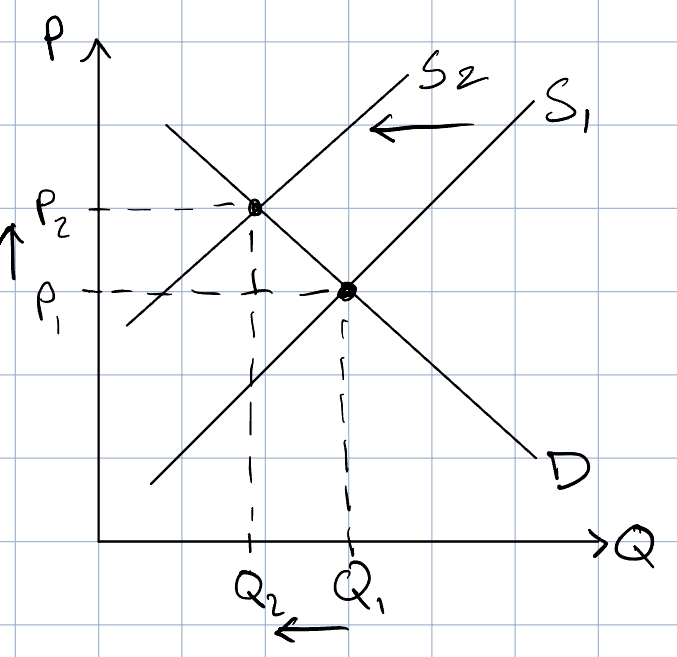
\includegraphics[width = 0.5\textwidth]{problem6b}
	\end{figure}
	
	\item The advancement in production technology will shift supply to the right which lowers the equilibrium price and raises the equilibrium quantity.
	\begin{figure}[h]
	\centering
	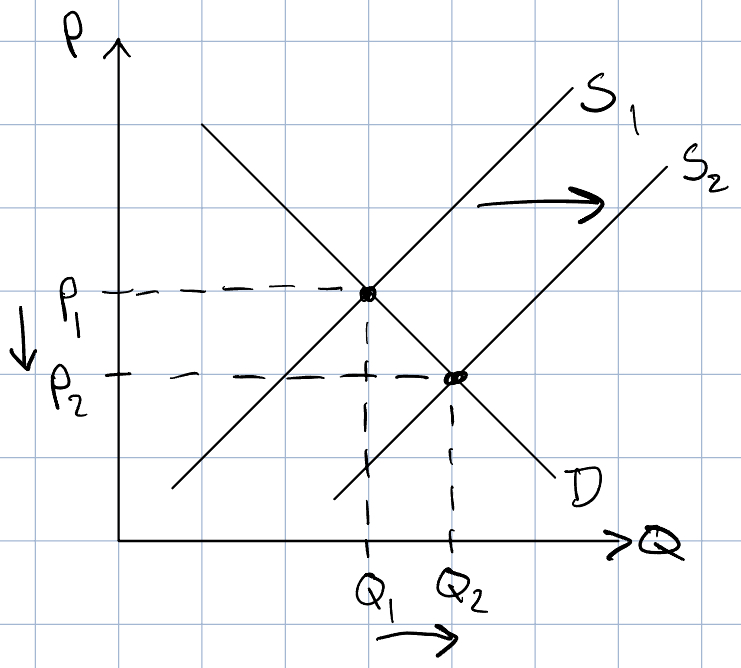
\includegraphics[width = 0.5\textwidth]{problem6c}
	\end{figure}
	
	\newpage
	
	\item SUVs are a substitute for minivans, so when they get more expensive, demand for minivans increases. That increases the equilibrium price and quantity of minivans.
	\begin{figure}[h]
	\centering
	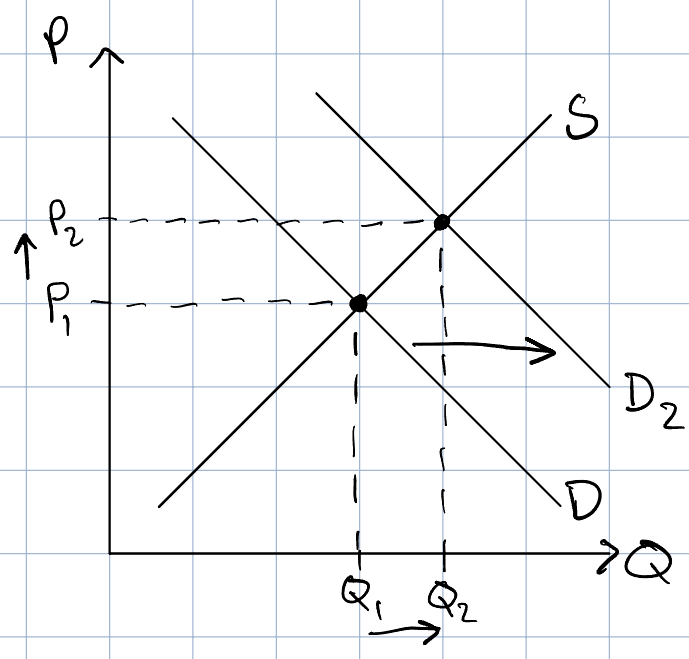
\includegraphics[width = 0.5\textwidth]{problem6d}
	\end{figure}
	
	\item Minivans are normal goods, so when incomes decline, people buy fewer minivans. That shifts demand to the left which lowers the equilibrium price and quantity. 
	\begin{figure}[h]
	\centering
	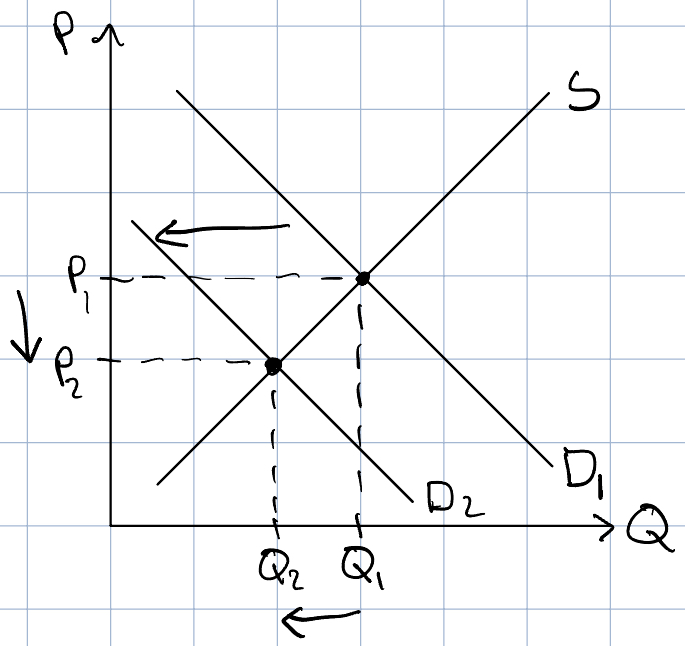
\includegraphics[width = 0.5\textwidth]{problem6e}
	\end{figure}
	
	\end{enumerate}
	
	\newpage
	
\item
	
	\begin{enumerate}
	
	\item The lower cost of manufacturing will shift the supply curve for TV screens to the right which decreases equilibrium price and increases equilibrium quantity.
	\begin{figure}[h]
	\centering
	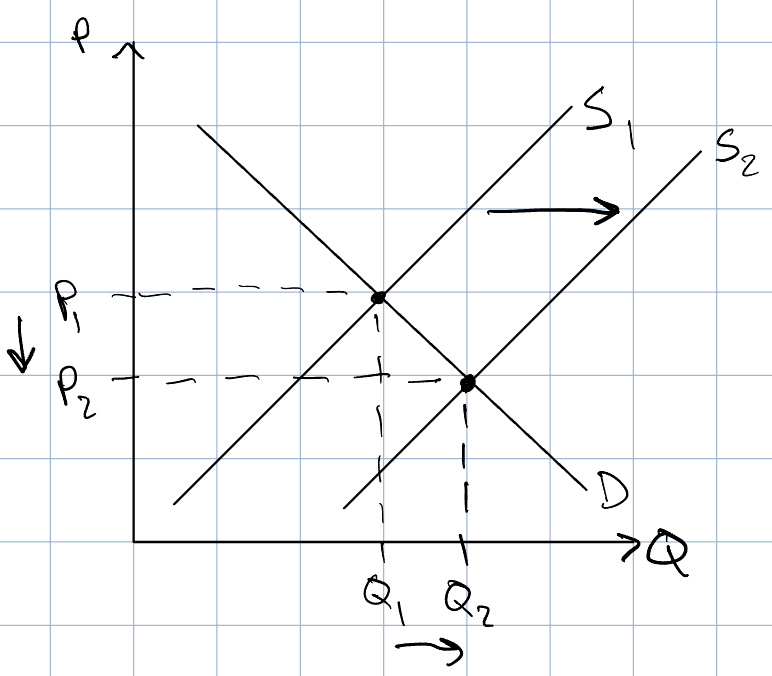
\includegraphics[width = 0.5\textwidth]{problem7a}
	\end{figure}
	
	\item Film streaming and TV screens are complements, so when the price of TV screens goes down, demand for streaming shifts right, price increases, and quantity increases.
	\begin{figure}[h]
	\centering
	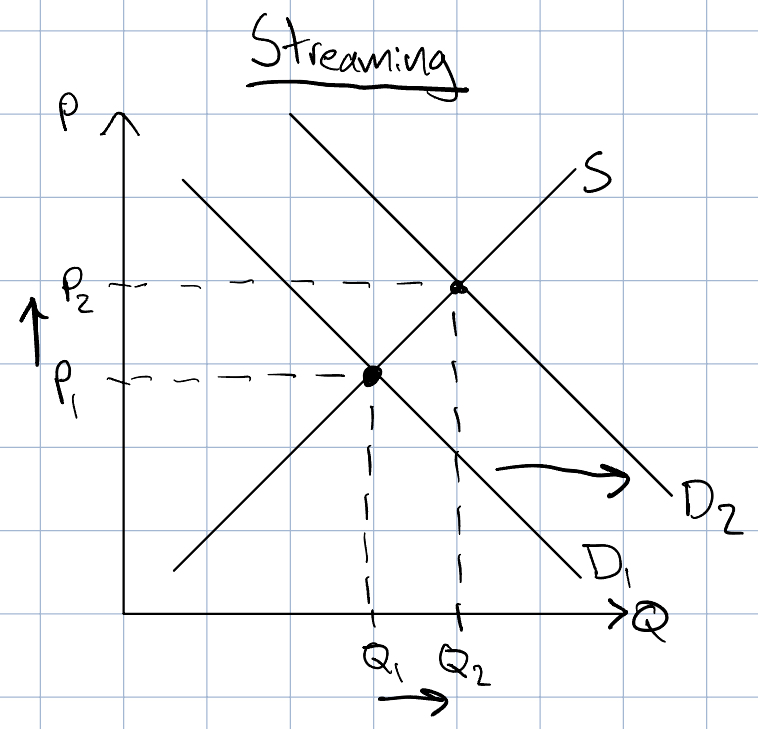
\includegraphics[width = 0.5\textwidth]{problem7b_streaming}
	\end{figure}
	
	Movie tickets and TV screens are substitutes, so when the price of TV screens goes down, demand for movie tickets shifts left, price decreases, and quantity decreases.
	\begin{figure}[h]
	\centering
	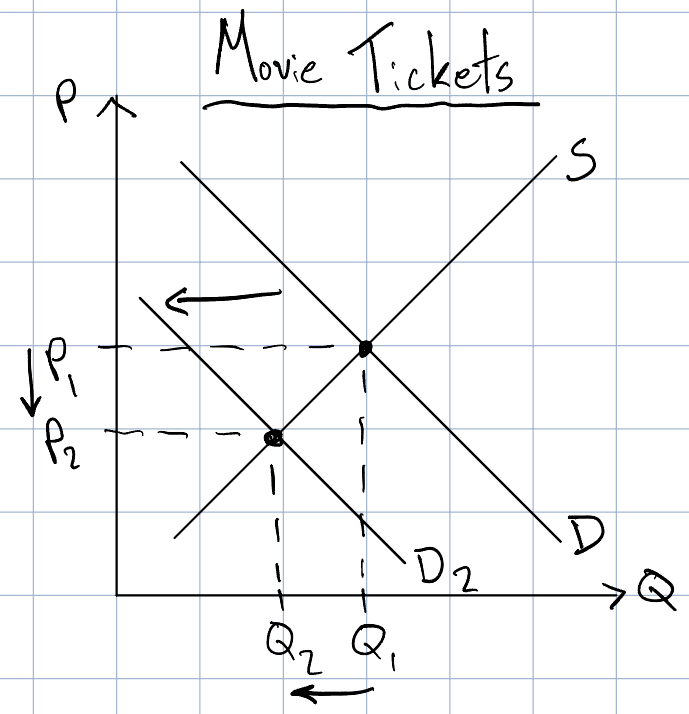
\includegraphics[width = 0.5\textwidth]{problem7b_tix}
	\end{figure}
	
	\end{enumerate}
	
\item

	\begin{enumerate}
	
	\item
	\begin{align*}
	Q_S &= Q_D \\
	4P^* &= 30 - 2P^* \\
	6P^* &= 30 \\
	P^* &= 5 \\
	\end{align*}
	
	\item
	\begin{align*}
	Q^* &= 4P^* \\
	Q^* &= 20
	\end{align*}
	
	\end{enumerate}

\end{enumerate}

\end{document}